\section{射影空间}\label{sec:projective-space}

初次接触射影簇时, 研究它的一个难点在于射影空间可以用许多不同方式定义. 这也正是它丰富而有趣之处. 我们将介绍射影空间的三种视角, 从最便于计算的一种开始.

\begin{Definition}{射影空间的第一种视角}\leavevmode\label{def:projective-space-homogeneous-coordinates}
设 $n\in\mathbb{N}$. $K$ 上的\emph{$n$ 维射影空间}, 记作 $\mathbb{P}_{K}^{n}$ 或简记为 $\mathbb{P}^{n}$, 是集合
\[
  \mathbb{P}^{n}=\frac{K^{n+1}\setminus\{(0,0,\ldots,0)\}}{\sim},
\]
其中 $\sim$ 是如下的等价关系:
\[
  \begin{gathered}
    (a_{0},a_{1},\ldots,a_{n})\sim(b_{0},b_{1},\ldots,b_{n})\\
    \Longleftrightarrow\\
    (\lambda a_{0},\lambda a_{1},\ldots,\lambda a_{n})=(b_{0},b_{1},\ldots,b_{n})
      \quad\text{对某个 }\lambda\in K\setminus\{0\}.
  \end{gathered}
\]
用 $[a_{0}:a_{1}:\cdots:a_{n}]$ 表示 $(a_{0},a_{1},\ldots,a_{n})$ 的等价类.
\end{Definition}

\BookPairedNoteLeft
  {注意, 在这一语境中, 目前只能把\textquotedbl{}维数\textquotedbl{}理解为对坐标个数的一种提示. 由于 $\mathbb{P}^{n}$ 既不是向量空间, 也不是仿射簇, 用本书到目前为止使用\textquotedbl{}维数\textquotedbl{}一词的任何一种意义, 都无法给 $\mathbb{P}^{n}$ 赋予有意义的维数.}
  {读者不妨停下来确认一下, $\sim$ 确实是等价关系.}
不过, 看过下列例子后, 我们使用\textquotedbl{}$n$ 维\textquotedbl{}这个术语可能就更容易理解了.

\begin{Example}{零维射影空间}\leavevmode\label{ex:zero-dimensional-projective-space}
$\mathbb{P}^{0}$ 的一个元素是等价类 $[a]$, 其中 $a\in K\setminus\{0\}$. 若对某个 $\lambda\in K\setminus\{0\}$ 有 $\lambda a=b$, 则 $[a]=[b]$. 特别地, 取 $\lambda=1/a$ 可知对任意 $a\in K\setminus\{0\}$ 都有 $[a]=[1]$, 所以 $\mathbb{P}^{0}$ 只有一个元素:
\[
  \mathbb{P}^{0}=\{[1]\}.
\]
\end{Example}

\begin{Example}{一维射影空间}\leavevmode\label{ex:one-dimensional-projective-space}
$\mathbb{P}^{1}$ 中的元素形如 $[a_{0}:a_{1}]$, 其中 $a_{0},a_{1}\in K$ 不全为零. 例如, $[1:2]$ 是 $\mathbb{P}^{1}$ 的一个元素. 把两个坐标同时乘以同一个 $\lambda\in K\setminus\{0\}$, 得到同一元素的不同表示:
\[
  [1:2]=[2:4]=[3:6]=[-1:-2]=\cdots.
\]
将 $\mathbb{P}^{1}$ 的元素分成两类很有启发性: 第一个坐标非零的, 以及第一个坐标为零的. 考虑第一类中的一个元素, 如 $[3:7]\in\mathbb{P}^{1}$. 将两个坐标同时乘以 $1/3$, 得
\[
  [3:7]=[1:7/3]\in\mathbb{P}^{1}.
\]
类似地, $\mathbb{P}^{1}$ 中第一个坐标非零的任何元素, 都对某个 $b\in K$ 等于 $[1:b]$. 另一方面, 第一个坐标为零的元素总等于 $[0:1]$. 例如, 将两个坐标同时乘以 $1/4$ 可知 $[0:4]=[0:1]\in\mathbb{P}^{1}$.

因此得到结论
\begin{equation}\label{eq:projective-line-coordinate-decomposition}
  \mathbb{P}^{1}=\{[1:b]\mid b\in K\}\sqcup\{[0:1]\}.
\end{equation}
\BookPairedNote
  {稍加思考就能看出, $b\neq b'$ 时, 两个元素 $[1:b]$ 与 $[1:b']$ 在 $\mathbb{P}^{1}$ 中不可能相等.}
  {用符号 $\sqcup$ 表示不交并. 换句话说, $A=B\sqcup C$ 表示 $A=B\cup C$ 且 $B\cap C=\varnothing$.}
因此, 形如 $[1:b]\in\mathbb{P}^{1}$ 的元素与 $\mathbb{A}^{1}$ 的元素之间有如下自然双射:
\[
  \begin{aligned}
    \{[1:b]\mid b\in K\}&\to\mathbb{A}^{1},\\
    [1:b]&\mapsto b.
  \end{aligned}
\]
在这个双射下, 分解 \eqref{eq:projective-line-coordinate-decomposition} 可以看成
\begin{equation}\label{eq:projective-line-affine-plus-one-point}
  \mathbb{P}^{1}=\mathbb{A}^{1}\sqcup\{[0:1]\}.
\end{equation}
\end{Example}

\begin{Example}{二维射影空间}\leavevmode\label{ex:two-dimensional-projective-space}
同上, $\mathbb{P}^{2}$ 的元素按第一个坐标非零还是为零分为两类. 第一个坐标非零的元素可以重新缩放为 $[1:b_{1}:b_{2}]$. 因此
\[
  \begin{aligned}
    \mathbb{P}^{2}={}&\{[1:b_{1}:b_{2}]\mid b_{1},b_{2}\in K\}\\
      &\sqcup\{[0:b_{1}:b_{2}]\mid b_{1},b_{2}\in K\text{ 不全为零}\}.
  \end{aligned}
\]
也与前例类似, 第一类元素与 $\mathbb{A}^{2}$ 有自然双射:
\[
  \begin{aligned}
    \{[1:b_{1}:b_{2}]\mid b_{1},b_{2}\in K\}&\to\mathbb{A}^{2},\\
    [1:b_{1}:b_{2}]&\mapsto(b_{1},b_{2}).
  \end{aligned}
\]
不过, 现在第一个坐标为零的元素不只一个, 而是有许多个. 例如 $[0:0:1]\neq[0:1:1]$. 实际上, $\mathbb{P}^{2}$ 中第一个坐标为零的元素与维数少一的射影空间有自然双射:
\[
  \begin{aligned}
    \{[0:b_{1}:b_{2}]\mid b_{1},b_{2}\in K\text{ 不全为零}\}&\to\mathbb{P}^{1},\\
    [0:b_{1}:b_{2}]&\mapsto[b_{1}:b_{2}].
  \end{aligned}
\]
在这两个双射下, 已经证明
\begin{equation}\label{eq:projective-plane-affine-plus-projective-line}
  \mathbb{P}^{2}=\mathbb{A}^{2}\sqcup\mathbb{P}^{1}.
\end{equation}
\end{Example}

分解 \eqref{eq:projective-line-affine-plus-one-point} 和 \eqref{eq:projective-plane-affine-plus-projective-line} 可以推广到任意 $n$, 这便引出射影空间的第二种视角.

\begin{Proposition}{射影空间的第二种视角}\leavevmode\label{prop:projective-space-affine-plus-infinity}
对任意 $n\geq1$, 有自然双射
\[
  \mathbb{P}^{n}=\mathbb{A}^{n}\sqcup\mathbb{P}^{n-1}.
\]
$\mathbb{P}^{n}$ 中属于 $\mathbb{P}^{n-1}$ 的元素称为 $\mathbb{P}^{n}$ 中的\emph{无穷远点}.
\end{Proposition}

证明这个双射是 Exercise~\ref{ex:projective-space-affine-part-and-infinity} 的内容. 如此前在 $\mathbb{P}^{1}$ 和 $\mathbb{P}^{2}$ 的情形所见, 关键是 $\mathbb{P}^{n}$ 中第一个坐标非零的元素对应于 $\mathbb{A}^{n}$ 的元素, 而第一个坐标为零的元素对应于 $\mathbb{P}^{n-1}$ 的元素.

但为何称为\textquotedbl{}无穷远点\textquotedbl{}? 为理解这一点, 考虑 $\mathbb{P}^{1}_{\mathbb{R}}$ 的情形. 在分解
\[
  \mathbb{P}^{1}_{\mathbb{R}}=\mathbb{A}^{1}_{\mathbb{R}}\sqcup\{[0:1]\}
\]
下, 元素 $1,2,3,\ldots\in\mathbb{A}^{1}_{\mathbb{R}}$ 对应于 $\mathbb{P}^{1}_{\mathbb{R}}$ 的下列元素:
\[
  [1:1],\ [1:2],\ [1:3],\ldots\in\mathbb{P}^{1}_{\mathbb{R}}.
\]
不过, 重新缩放可将它们表示为
\[
  \bigl[\tfrac{1}{1}:1\bigr],\ \bigl[\tfrac{1}{2}:1\bigr],\
  \bigl[\tfrac{1}{3}:1\bigr],\ldots\in\mathbb{P}^{1}_{\mathbb{R}}.
\]
\BookPairedNote
  {因此, 随着 $n\in\mathbb{A}^{1}_{\mathbb{R}}$ 任意增大, $\mathbb{P}^{1}_{\mathbb{R}}$ 中对应的点 $[\frac{1}{n}:1]$ 趋于 $[0:1]$. 这就解释了为什么称 $[0:1]$ 为\emph{无穷远点}, 并写成}
  {这里在 $\mathbb{P}^{n}$ 中使用\textquotedbl{}极限\textquotedbl{}只是直观上的说法, 要精确定义极限还需要拓扑.}
\[
  \mathbb{P}^{1}_{\mathbb{R}}=\mathbb{A}^{1}_{\mathbb{R}}\sqcup\{\infty\}.
\]
注意, 当 $n\to\infty$ 时, $-n\in\mathbb{A}^{1}_{\mathbb{R}}$ 对应的 $[1:-n]\in\mathbb{P}^{1}_{\mathbb{R}}$ 也趋于 $[0:1]$. 因此, 将 $\mathbb{P}^{1}_{\mathbb{R}}$ 画成\hyperref[fig:projective-real-line-loop]{下图的环形}很有助于理解: 沿 $\mathbb{A}^{1}_{\mathbb{R}}$ 的任一方向走得任意远, 都趋于同一个点 $[0:1]\in\mathbb{P}^{1}_{\mathbb{R}}$.
\par\smallskip
{\centering\phantomsection\label{fig:projective-real-line-loop}%
  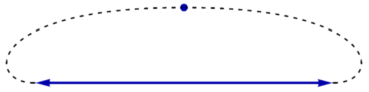
\includegraphics[width=.55\linewidth]{figures/projective-real-line-loop.pdf}\par}

对 $n>1$, 要画出 $\mathbb{P}^{n}$ 的直观图形会更难, 但同样的视角仍然成立. 例如, 有
\[
  \mathbb{P}^{2}_{\mathbb{R}}=\mathbb{A}^{2}_{\mathbb{R}}\sqcup\{\text{无穷远点}\}.
\]
在这个空间中, 可以沿 $\mathbb{A}^{2}_{\mathbb{R}}$ 中任意直线趋向无穷远. 为此, 考虑沿斜率为 $m$, $y$ 轴截距为 $b$ 的直线 $y=mx+b$ 向外延伸的点列 $(1,m+b),(2,2m+b),(3,3m+b),\ldots$. 这些点在 $\mathbb{P}^{2}_{\mathbb{R}}$ 中对应于
\[
  [1:1:m+b],\ [1:2:2m+b],\ [1:3:3m+b],\ldots\in\mathbb{P}^{2}_{\mathbb{R}}.
\]
重新缩放后, 得到等价的点
\[
  \bigl[\tfrac{1}{1}:1:m+\tfrac{b}{1}\bigr],\
  \bigl[\tfrac{1}{2}:1:m+\tfrac{b}{2}\bigr],\
  \bigl[\tfrac{1}{3}:1:m+\tfrac{b}{3}\bigr],\ldots\in\mathbb{P}^{2}_{\mathbb{R}},
\]
它们趋向 $[0:1:m]$. 这个极限是 $\mathbb{P}^{2}_{\mathbb{R}}$ 的一个\textquotedbl{}无穷远点\textquotedbl{}, 因为它的第一个坐标为零. \hyperref[fig:projective-real-plane-infinity]{下图}画出了 $\mathbb{A}^{2}_{\mathbb{R}}$ 和 $\mathbb{P}^{2}_{\mathbb{R}}$ 中沿不同斜率的直线所趋近的几个无穷远点.

\BookPairedFigure
  {现在可以看出, 为什么 $\mathbb{P}^{2}_{\mathbb{R}}$ 有许多无穷远点, 而 $\mathbb{P}^{1}_{\mathbb{R}}$ 只有一个: 在 $\mathbb{P}^{2}_{\mathbb{R}}$ 中沿直线向外走时, 所趋近的无穷远点取决于这条直线的斜率. 实际上, 可以把\textquotedbl{}沿直线走向它所通往的无穷远点\textquotedbl{}的想法精确表述为一个双射: $\mathbb{P}^{2}_{\mathbb{R}}$ 中的无穷远点对应于 $\mathbb{A}^{2}_{\mathbb{R}}$ 中经过原点的直线. 这是一个更一般现象的特例, 下面给出陈述.}
  {\phantomsection\label{fig:projective-real-plane-infinity}%
   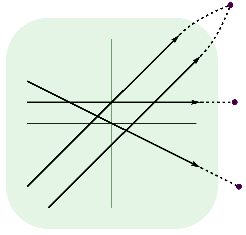
\includegraphics[width=\linewidth]{figures/projective-real-plane-infinity.pdf}}

\begin{Proposition}{无穷远点是直线的斜率}\leavevmode\label{prop:points-at-infinity-correspond-to-lines-through-origin}
对任意 $n\in\mathbb{N}$, 有自然双射
\[
  \{\mathbb{P}^{n}\text{ 中的无穷远点}\}
    =\{\mathbb{A}^{n}\text{ 中经过 }(0,\ldots,0)\text{ 的直线}\}.
\]
\end{Proposition}
\begin{Proof}
按定义, 经过 $(0,\ldots,0)\in\mathbb{A}^{n}$ 的直线是形如
\[
  L=\{(\lambda a_{1},\lambda a_{2},\ldots,\lambda a_{n})\mid\lambda\in K\}
\]
的点集, 其中 $a_{i}\in K$ 固定, 且至少一个 $a_{i}$ 非零. 所需的双射就是把直线
\[
  L=\{(\lambda a_{1},\lambda a_{2},\ldots,\lambda a_{n})\mid\lambda\in K\}
\]
对应到无穷远点
\[
  [0:a_{1}:a_{2}:\cdots:a_{n}]\in\mathbb{P}^{n}.
\]
可将该点看成 $L$ 上向外延伸的点列所趋向的点 (建议读者从直观上验证).
\end{Proof}

由于 $\mathbb{P}^{n}$ 的无穷远点也与 $\mathbb{P}^{n-1}$ 双射, 可以从另一个角度看 Proposition~\ref{prop:points-at-infinity-correspond-to-lines-through-origin}: 它给出了射影空间的第三种视角, 这种视角常被用作射影空间本身的另一种定义.

\begin{Corollary}{射影空间的第三种视角}\leavevmode\label{cor:projective-space-as-lines-through-origin}
对任意 $n\in\mathbb{N}$, 有自然双射
\[
  \mathbb{P}^{n}=\{\mathbb{A}^{n+1}\text{ 中经过 }(0,\ldots,0)\text{ 的直线}\}.
\]
\end{Corollary}

沿 Proposition~\ref{prop:points-at-infinity-correspond-to-lines-through-origin} 的双射追溯, 可以看出怎样将第一种和第三种视角对应起来: 元素 $[a_{0}:a_{1}:\cdots:a_{n}]\in\mathbb{P}^{n}$ 对应于直线
\[
  L=\{(\lambda a_{0},\lambda a_{1},\ldots,\lambda a_{n})\mid\lambda\in K\}\subseteq\mathbb{A}^{n+1},
\]
即经过原点和 $(a_{0},a_{1},\ldots,a_{n})\in\mathbb{A}^{n+1}$ 的直线.

将这些想法合起来, 可以从三种角度看 $\mathbb{P}^{n}$ 的元素: 它是一个等价类 $[a_{0}:a_{1}:\cdots:a_{n}]$, 是 $\mathbb{A}^{n}$ 中的一个点或一个无穷远点, 或者是 $\mathbb{A}^{n+1}$ 中经过原点的一条直线. 根据语境在这些视角之间自如切换, 正是读者在探索射影空间, 以及从下一节开始探索已知的簇的理论在射影空间中的对应理论时, 将逐渐掌握的能力之一.

\BookExerciseHeading
\begin{BookExercises}
  \item\label{ex:compare-projective-coordinate-representatives} 设 $[2:1:3]\in\mathbb{P}^{2}$. 证明
  \[
    [2:1:3]=[6:3:9]
  \]
  但
  \[
    [2:1:3]\neq[6:4:12].
  \]
  一般地, 哪些 $[a:b:c]\in\mathbb{P}^{2}$ 满足 $[2:1:3]=[a:b:c]$?
  \item\label{ex:cross-multiplied-projective-coordinates} 证明 $[a_{0}:\cdots:a_{n}]=[b_{0}:\cdots:b_{n}]\in\mathbb{P}^{n}$ 当且仅当
  \[
    a_{i}b_{j}=a_{j}b_{i}\qquad\text{对所有 }i,j\in\{0,\ldots,n\}.
  \]
  在这种情形, 称交叉相乘的结果相同.
  \item\label{ex:projective-space-affine-part-and-infinity} 分三步证明存在自然双射 $\mathbb{P}^{n}=\mathbb{A}^{n}\sqcup\mathbb{P}^{n-1}$:
  \begin{enumerate}
    \item 定义
    \[
      U=\{[a_{0}:a_{1}:\cdots:a_{n}]\in\mathbb{P}^{n}\mid a_{0}\neq0\}
    \]
    和
    \[
      V=\{[a_{0}:a_{1}:\cdots:a_{n}]\in\mathbb{P}^{n}\mid a_{0}=0\}.
    \]
    证明 $\mathbb{P}^{n}=U\sqcup V$.
    \item 证明 $U$ 与 $\mathbb{A}^{n}$ 之间有自然双射.
    \item 证明 $V$ 与 $\mathbb{P}^{n-1}$ 之间有自然双射.
  \end{enumerate}
  \item\label{ex:projective-space-disjoint-affine-decomposition} 证明存在自然双射
  \[
    \mathbb{P}^{n}=\mathbb{A}^{n}\sqcup\mathbb{A}^{n-1}\sqcup\mathbb{A}^{n-2}
      \sqcup\cdots\sqcup\mathbb{A}^{1}\sqcup\mathbb{A}^{0}
  \]
  并描述每个分量中的点.
  \item\label{ex:projective-point-affine-and-line-perspectives} 设 $[2:1:3]\in\mathbb{P}^{2}$. 将这个点描述成
  \begin{enumerate}
    \item $\mathbb{A}^{2}\sqcup\mathbb{P}^{1}$ 的一个元素;
    \item $\mathbb{A}^{3}$ 中经过 $(0,0,0)$ 的一条直线.
  \end{enumerate}
  \item\label{ex:projective-infinity-point-affine-and-line-perspectives} 对点 $[0:1:3]\in\mathbb{P}^{2}$ 重做 Problem~\ref{ex:projective-point-affine-and-line-perspectives}.
  \item\label{ex:origin-lines-projecting-to-infinity} $\mathbb{A}^{3}$ 中经过 $(0,0,0)$ 的哪些直线对应于 $\mathbb{P}^{2}$ 中的无穷远点?
\end{BookExercises}
